\documentclass{report}

\usepackage[italian]{babel} % Imposta la lingua italiana
\usepackage{tcolorbox}
\usepackage{forest}
\usepackage{dirtree} % Aggiungi il pacchetto dirtree
\usepackage{graphicx} % Aggiungi il pacchetto graphicx
\usepackage{amsmath}
\usepackage{pgfplots}
\usepackage{tikz}
\usepackage{hyperref}
\hypersetup{
    colorlinks=true,
    linkcolor=black,
    filecolor=magenta,      
    urlcolor=cyan,
    pdftitle={Overleaf Example},
    pdfpagemode=FullScreen,
    }
\pgfplotsset{width=5cm,compat=1.9}

\renewcommand{\thefootnote}{\roman{footnote}}
% Definizione del nuovo ambiente 'important'
\newtcolorbox{important}[1][]{
  colback=yellow!10!white,
  colframe=red!50!black,
  title=Ricorda,
  #1
}

\begin{document}

\begin{center}
  \vspace*{2cm}
  {\Huge Probabilità e statistica \par}
  \vspace{1cm}
  
\includegraphics[width=0.5\textwidth]{logounibs.png}\par
  \vspace{1cm}
  {\Large Riccardo Rasori \par}
  \vspace{0.5cm}
  {\large A.A. 2024/2025 \par}
  \vspace{2cm}
\end{center}

\tableofcontents % Aggiungi l'indice


\section{Calcolo combinatorio}
\begin{itemize}
  \item Dati n oggetti distinti\\Si dicono \textbf{distinzioni semplici} tutti i gruppi che si formano con k elementi in modo che i gruppi differiscano
        \begin{itemize}
          \item O per l'ordine
          \item O per almeno un elemento
        \end{itemize}
        $\Delta_{n,k} = n*(n-1)*...*(n-k+1)*\frac{(n-k)!}{(n-k)!}=\frac{n!}{(n-k)!}$\\
        Es. n=4, k=2 A=\{1,5,3,8\}\\ $\Delta_{4,2} = \frac{4!}{2!}=12$
  \item Si dicono \textbf{disposizioni con ripetizioni} di classe k tutti i gruppi che si possono formare con k elementi on la possibilità che gli elementi si ripetano in un gruppo in modo che due gruppi differiscano
        \begin{itemize}
          \item Per ordine
          \item Per almeno un elemento  $\Delta_{n,k}^* = n^k$
          \item Per ripetizione
        \end{itemize}
        Es. k=2, n=4 A=\{1,5,3,8\}\\ $\Delta_{n,k} = n^k = 4^2 = 16$
  \item Dati n oggetti distinti si dicono \textbf{permutazioni semplici} di n elementi i gruppi che si riescono a formare con n elementi in modo che due gruppi differiscano
        \begin{itemize}
          \item Per l'ordine di elementi
        \end{itemize}
        $P_n=\Delta_{n,n} = n!$\\
        Es. 3 persone su 3 posti $\Rightarrow$ 3!
  \item Si dicono \textbf{combinazioni semplici} di n oggetti di classe k tutti i gruppi formati con k degli n elementi in modo che due gruppi differiscano
        \begin{itemize}
          \item Per almeno un elemento
        \end{itemize}
        $C_{n,k} = \frac{\Delta_{n,k}}{P_k} = \frac{n!}{k!(n-k)!}=\binom{n}{k}$\\
        Es. Ho 4 liquori, quanti biberoni ottengo mescolandone 3 alla volta?\\
        $C_{4,3} = \binom{4}{3} = \frac{4!}{3!(4-3)!} = 4$\\
        \\
        Es. Ho 5 oggetti da mettere in 3 scatole\\
        k=5, n=3\\
        In quanti modi posso fare?\\
        Disegnamo una possibile configurazione
        \begin{center}
          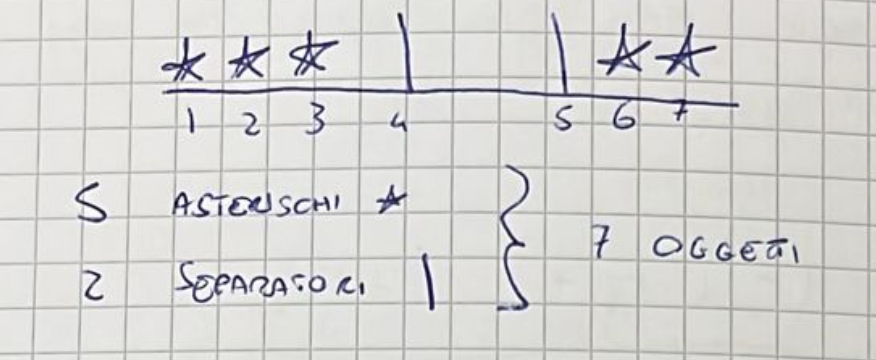
\includegraphics[scale=0.25]{img1.png}
        \end{center}
        $\frac{7!}{5!2!} = 21$\\
        Quindi ho $\frac{(n+k-1)!}{k!(n-1)!}=\binom{n+k-1}{k}=C_{n+k-1,k}$\\
        Sono \textbf{combinazioni di} n oggetti \textbf{con ripetizione} di classe k tutti i gruppi formati con l degli n elementi con la possibilità di ripetizioni in modo che differiscano per:
        \begin{itemize}
          \item ...
          \item ...
          \item ...
        \end{itemize}
        Es. Sia $A=\{\Delta,\bigotimes\}$ quante sequenze di 3 simboli posso fare?\\
        $C_{2,3}^* = \binom{4}{3} = \frac{4!}{3!(4-3)!} = 4$
  \item Dati n oggetti con $r_1$ oggetti uguali tra loro e $r_2$ oggetti uguali con\\
        $r_1+r_2+...+r_k=n$\\
        Sono \textbf{permutazioni con ripetizione} i gruppi formati con alcuni elementi indistinguibili tra loro in modo che i gruppi differiscano per:
        \begin{itemize}
          \item l'ordine\\
        \end{itemize}
        \begin{center}
          $P_{r_1,r_2,...,r_k} = \frac{r_1+r_2+...+r_k}{r_1!r_2!...r_k!}$
        \end{center}
        Es. Anagrammi di ``AFA"\\
        $r_1=2, r_2=1$\\
        $P_{2,1} ^* = \frac{3!}{2!1!} = 3$\\
        Es. Urna con 40 numeri distinti e 6 estrazioni, quante combinazioni posso fare?\\
        \begin{itemize}
          \item Estrazione senza reinserimento e conta la sequenza\\$\Delta_{40,6} = \frac{40!}{6!(40-6)!} = 3.838.380$
          \item Senza reinserimento e non conta la sequenza\\$C_{40,6} = \binom{40}{6}$
          \item Con reinserimento e conta la sequenza\\$\Delta_{40,6}^* = 40^6$
          \item Con reinserimento e non conta la sequenza\\$C_{40,6}^* = \binom{40+6-1}{6}=\binom{45}{6}$
        \end{itemize}
        Es. 4 persone, 5 posti numerati\\
        n=5, k=4\\
        $\Delta_{5,4}=\frac{(5-4)!}{1!} = 5! = 120$\\
        Es. A=\{1,2,3,4,5,6,7,8,9\} \\
        \begin{itemize}
          \item Quanti numeri di 3 cifre distinte?\\k=3 $9*8*7$
          \item Quanti numeri sono dispari?\\$5*8*7$
          \item Quanti terminano con 9?\\$\Delta_{8,2}=8*7*1$
          \item Quanti numeri sono maggiori di 700?\\$8*7*3$
        \end{itemize}
        Es. A=\{1,2,3,4,5,6,7,8,9\}
        \begin{itemize}
          \item Quanti numeri di 3 cifre anche ripetute?\\$\Delta_{9,3}^* = 9^3$
          \item Quanti numeri sono dispari?\\$\Delta_{9,2}^* = 9^2*5$
          \item Quanti maggiori di 700?\\$\Delta_{9,2}^* = 9^2*3$
        \end{itemize}
        Es. Tema esame\\
        Urnca con 9 palline, 3 hanno ``1", 3 ``2", 3 ``3"\\
        Estraggo senza reimmissione\\
        Quanti numeri di 9 cifre diversi posso fare?\\
        $P_{3,3,3}^* = \frac{9!}{3!3!3!}$\\
        Es. 5 particelle con spin $s=\frac{1}{2}$ orientato in posizione up $\uparrow$ o down $\downarrow$\\
        Le particelle non interagiscono tra loro
        \begin{itemize}
          \item Quante configurazioni posso fare con 3 spin up?\\n=5, k=3\\$C_{5,3} = \binom{5}{3}=\frac{5!}{3!2!}=10$
          \item E con 2 spin up\\k=2\\$C_{5,2} = \binom{5}{2}=\frac{5!}{2!3!}=10$
        \end{itemize}
        Es. Nel circuito in figura gli interruttori ($I_i,i=1,2,3,4$) sono aperti o chiusi, quante configurazioni fanno passare la corrente da A a B\\
        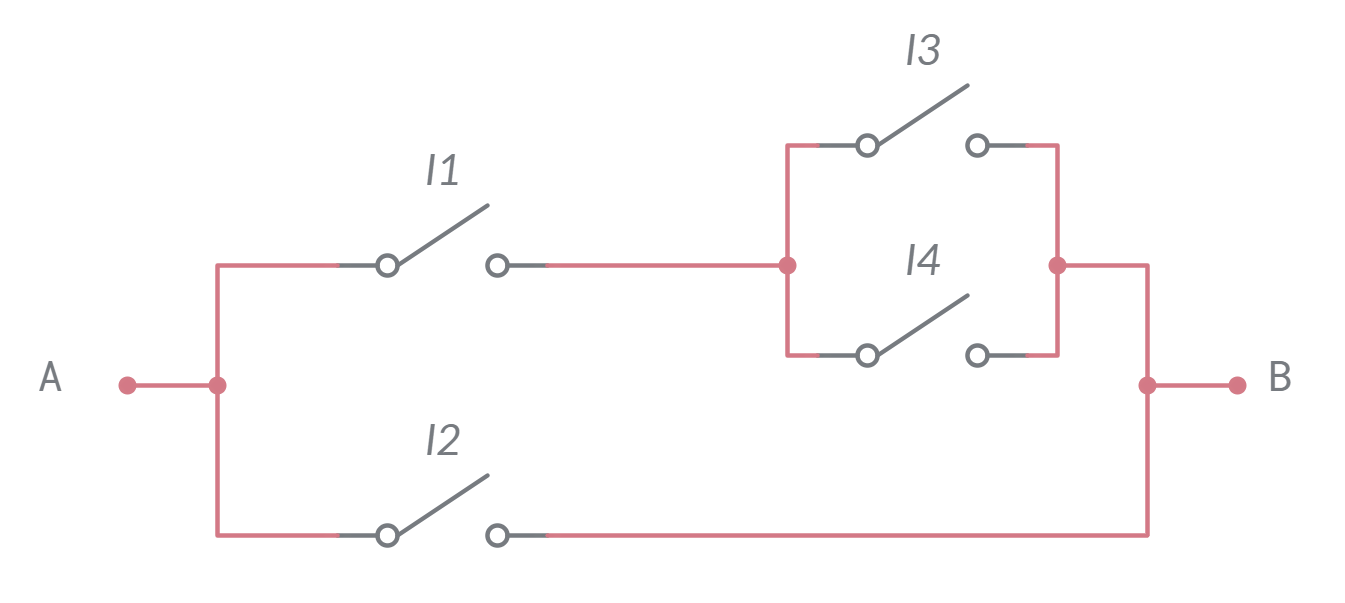
\includegraphics[scale=0.3]{img2.png}
        $1*2^3+1*1*[4-1]=11$\\
        $\Delta_{1,1}^* * \Delta_{2,3}^* + \Delta_{1,1}^* * \Delta_{1,1}^* [\Delta_{2,2}^*-\Delta_{1,2}^*]$
        \\
        Es. 10 abiti, 5 paia di scarpe, 2 cappelli\\
        $C_{10,1}*C_{5,1}*C_{2,1}=10*5*2=100$
\end{itemize}


\end{document}